\documentclass[11pt, a4paper, leqno]{article}
\usepackage{a4wide}
\usepackage[T1]{fontenc}
\usepackage[utf8]{inputenc}
\usepackage{float, afterpage, rotating, graphicx}
\usepackage{epstopdf}
\usepackage{longtable, booktabs, tabularx}
\usepackage{fancyvrb, moreverb, relsize}
\usepackage{eurosym, calc}
% \usepackage{chngcntr}
\usepackage{amsmath, amssymb, amsfonts, amsthm, bm}
\usepackage{caption}
\usepackage{mdwlist}
\usepackage{xfrac}
\usepackage{setspace}
\usepackage[table]{xcolor}
\usepackage{subcaption}
\usepackage{minibox}
\usepackage{tocloft}
% \usepackage{pdf14} % Enable for Manuscriptcentral -- can't handle pdf 1.5
% \usepackage{endfloat} % Enable to move tables / figures to the end. Useful for some submissions.


\usepackage[
    natbib=true,
    bibencoding=inputenc,
    bibstyle=authoryear-ibid,
    citestyle=authoryear-comp,
    maxcitenames=3,
    maxbibnames=10,
    useprefix=false,
    sortcites=true,
    backend=biber
]{biblatex}
\AtBeginDocument{\toggletrue{blx@useprefix}}
\AtBeginBibliography{\togglefalse{blx@useprefix}}
\setlength{\bibitemsep}{1.5ex}
\addbibresource{refs.bib}


\usepackage[unicode=true]{hyperref}
\hypersetup{
    colorlinks=true,
    linkcolor=black,
    anchorcolor=black,
    citecolor=black,
    filecolor=black,
    menucolor=black,
    runcolor=black,
    urlcolor=blue
}

\usepackage{array}
\newcolumntype{L}{>{\centering\arraybackslash}m{4.5cm}}

\widowpenalty=10000
\clubpenalty=10000

\setlength{\parskip}{1ex}
\setlength{\parindent}{0ex}
\setstretch{1.5}

\renewcommand*\contentsname{Table of Contents}

\begin{document}

\title{Visualizating Covid-19 Contact Restriction Policies in Germany\thanks{Emily Anne Schwab, Satwika Vysetty , University of Bonn. Email: \href{mailto:s6emschw@uni-bonn.de, s6savyse@uni-bonn.de}{\nolinkurl{s6emschw [at] uni-bonn [dot] de, s6savyse [at] uni-bonn [dot] de}}.}}

\author{Emily Anne Schwab, Satwika Vysetty}

\date{
    {\bf Preliminary -- please do not quote}
    \\[1ex]
    \today
}

\maketitle

\pagenumbering{roman}

\begin{abstract}
As a result of the Covid-19 pandemic, governments around the world implemented an array of policy measures to alleviate the enormous strains placed on their country’s healthcare systems and to mitigate the pandemic’s economic consequences for businesses and households alike. Since shortcomings in modern epidemiological models make it difficult to study the potential effects of these policies imposed during the Covid-19 health crisis, researchers at the Bonn Graduate School of Economics (BGSE) and the Institute of Labor Economics (IZA) developed a unique simulation model using agent-based theory to study the social and economic costs of such dynamic policy measures. By understanding the spread of Covid-19 through social contacts as well as the impact of various social distancing policies on reducing the infection and death rates associated with the virus, the research team’s work can assist governments in determining which policy measures are most effective in minimizing negative social and economic outcomes of the pandemic.

For our final project in Effective Programming Practices for Economists (EPP), we collaborated with members of the research team to create a data set tracking the stringency level of social distancing policies recommended by the German federal government. The data entries for the policy measures begin approximately a month before the start of the first lockdown period, on February 15, 2020 and end a year later on February 14, 2021. In order to capture the stringency level of contact restriction measures that affect various forms of daily social encounters, our data set differentiates between policies that target the education system, private gathering, and public activities such as shopping and entertainment. Upon completing our data set and producing an individual stringency index for each social contact category as well as an aggregate stringency index, we employed mobility data from the Google Covid-19 Community Mobility Reports to produce visualizations that reveal the effects of Germany’s Covid-19 lockdown policies to daily forms of social contact.
\end{abstract}
\clearpage

\tableofcontents
\clearpage

%\listoffigures
%\clearpage

\pagenumbering{arabic}

\addcontentsline{toc}{section}{Introduction}
\section*{Introduction} % (fold)
\label{sec:introduction}

%If you are using this template, please cite this item from the references: \citet{GaudeckerEconProjectTemplates}

%\citet{Schelling69} example in the code is taken from \citet{StachurskiSargent13}

As a result of the Covid-19 pandemic, governments around the world implemented an array of policy measures to alleviate the enormous strains placed on their country’s healthcare systems and to mitigate the pandemic’s economic consequences for businesses and households alike. Since shortcomings in modern epidemiological models make it difficult to study the potential effects of these policies imposed during the Covid-19 health crisis, researchers at the Bonn Graduate School of Economics (BGSE) and the Institute of Labor Economics (IZA) developed a unique simulation model using agent-based theory to study the social and economic costs of such dynamic policy measures. By understanding the spread of Covid-19 through social contacts as well as the impact of various social distancing policies on reducing the infection and death rates associated with the virus, the research team’s work can assist governments in determining which policy measures are most effective in minimizing negative social and economic outcomes of the pandemic.

For our final project in Effective Programming Practices for Economists (EPP), we collaborated with members of the research team to create a data set tracking the stringency level of social distancing policies recommended by the German federal government. The data entries for the policy measures begin approximately a month before the start of the first lockdown period, on February 1, 2020 and end a year later on February 14, 2021. In order to capture the stringency level of contact restriction measures that affect various forms of daily social encounters, our data set differentiates between policies that target the education system, private gathering, and public activities such as shopping and entertainment. Upon completing our data set and producing an individual stringency index for each social contact category as well as an aggregate stringency index, we employed mobility data from the Google Covid-19 Community Mobility Reports to produce visualizations that reveal the effects of Germany’s Covid-19 lockdown policies to daily forms of social contact.

In section 1 of the following report, we will begin with an explanation of the data gathering and management process. We will then discuss the mathematical derivation of our stringency indices in section 2. Section 3 will entail a summary of our visualizations and a subsequent analysis of their implications. Finally, we will provide concluding remarks.

%\begin{figure}
   % \caption{Segregation by cycle in the baseline \citet{Schelling69} model as in the \citet{StachurskiSargent13} example}

    %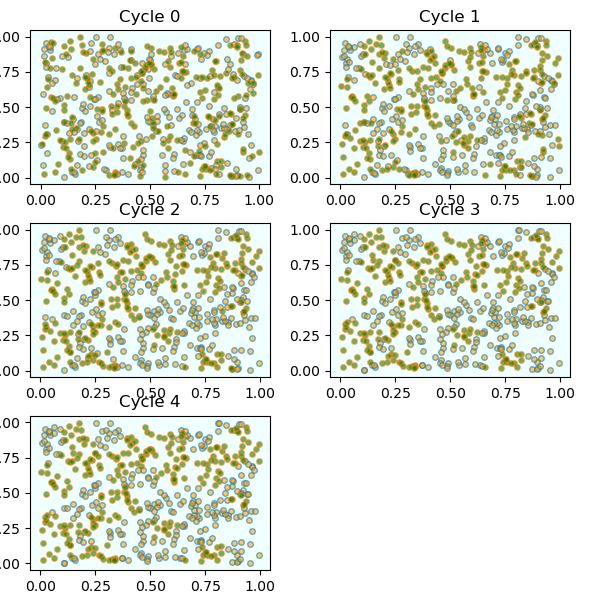
\includegraphics[width=\textwidth]{../../bld/figures/schelling_baseline}

%\end{figure}


%\begin{figure}
   % \caption{Segregation by cycle in the baseline \citet{Schelling69} model, limiting the number of potential moves per period to two}

    %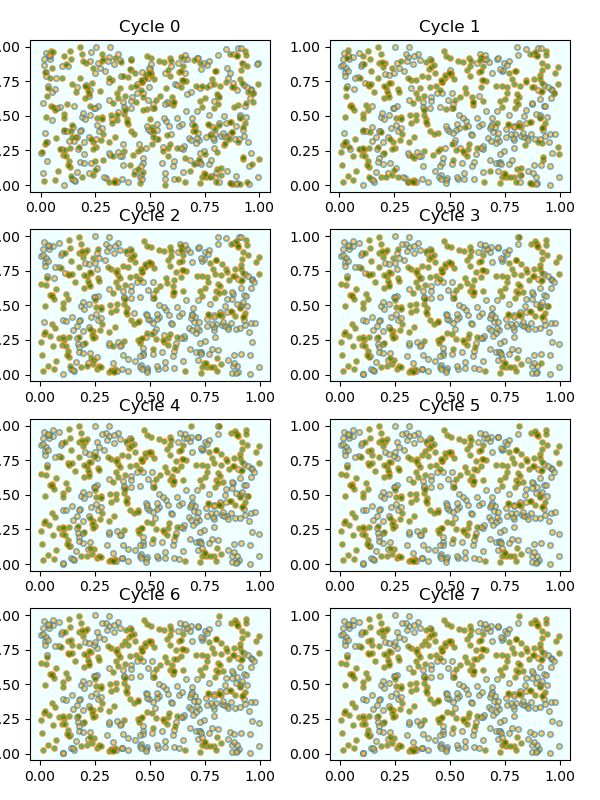
\includegraphics[width=\textwidth]{../../bld/figures/schelling_max_moves_2}

%\end{figure}

% section introduction (end)

\section{Data Gathering and Management} % (fold)
\label{sec:section1}

In order to obtain accurate information on any changes to social distancing policies announced by the German federal government, we searched through press releases concerning the developments of the Covid-19 outbreak published on the federal government website between February 2020 and February 2021. Given the dynamic nature of the government’s contact restrict measures, with policy adjustments announced every two to four weeks depending on the infection incidence level, we track the start and end date for each policy. While these official policy announcements carefully outlined regulations that restricted a wide range of daily public and private social encounters, our data set is limited to policy measures that influence social contact in schools, private gatherings, and public activities.

For each policy, we include a description of the measure, which is later used to create an ordinal scale of measurement that reports the restrictiveness of the policy. Also relevant is whether each policy is implemented federally or by an individual state. As time restrictions did not permit us to include state-level contact restriction policies, all entries in the existing data set track the suggested policy measures announced by the federal government. We additionally distinguish between policies that directly affect social contact in schools and those that impact other forms of contact including private gatherings and public activities. Finally, each entry includes links to the federal press release pages that announce the dates on which a given policy begins and ends.

In order to generate a representative account of the German school system, we produced sub-index score indicators that differentiate between four distinct grade levels including early childcare (E1), elementary school (E2), grades 5 to 10 (E3), and grades 11 to 12/13 (E4). We then repeated a similar procedure to observe aspects of public activities and private gatherings, respectively. To capture the effects of Covid-19 social distancing policies on public activities, we generated an additional four indicators to track restrictions on stores (S1), restaurants (S2), entertainment, sports and cultural facilities (S3), and finally religious gatherings (S4). Restrictions on private gatherings were summarized into a single indicator (R1), which observes the limitations on the number of individuals and/or households that may visit with each other at any given time.

After these preliminary efforts, we then used ordinal scales of measurement to rank stringency level for the individual policy phases of each sub-index score indicator. While the ordinal scales created for each indicator vary in terms of their maximum value, a value of zero always indicates no contact restriction; values of 1 or larger represent an increase in the policy’s level of contact stringency. For descriptions of the sub-index score indicators and their respective numerical scales, please view the codebook we provide as a separate document. The data set further assigns each policy entry three additional values, namely two binary variables, the flag and the recorded flag, as well as the maximum value of the policy’s affiliated indicator. While the flag variable distinguishes between indicators that are not characterized by their geographic scope (0) and those that are (1), the recorded flag indicates whether an indicator was implemented at the state (0) or national (1) level.

% section1 (end)

\section{Calculating the Indicator Sub-index Scores and Resulting Stringency Indices} % (fold)
\label{sec:section2}

After completing the data gathering process and producing the subsequent data set, we employed a simple computational procedure inspired by the one used by the Oxford Covid-19 Government Response Tracker to calculate a daily sub-index score for each of our nine indicators. In order to calculate the sub-index scores ($I$) for a given indicator ($j$) on a particular day ($t$), we use the following formula:

\begin{equation}\label{eq:Eq1}
  I_{j,t} = 100\frac{v_{j,t} - 0.5\left(F_j - f_{j,t}\right)}{N_j}
\end{equation}

where $v_{j,t}$ is the ordinal value assigned to a policy affiliated with the $j$-th indicator, $N_j$ represents the maximum possible value of the indicator, Fj is the binary variable identifying whether the indicator has a flag variable, and $f_{j,t}$ is the recorded binary flag of the indicator. The formula yields a normalized sub-index value between 0 and 100, which accounts for the differing ordinal measurement scales of the individual indicators. In the case that an indicator uses a flag variable and the recorded flag for a given policy is 0, suggesting that the policy targets only a small region, then the formula subtracts a half point from the ordinal value to reduce the level of stringency associated with the policy measure. Note that if there is no policy implemented for a given indicator (that is, if the ordinal value $v_{j,t}$ is 0), \text{then the function}  $\left(F_{j} - f_{j,t}\right)$ is also treated as 0, yielding a sub-index score ($I_{j,t}$) of zero.

Using the daily sub-index scores computed for each indicator, we produce stringency indices that measure the restrictiveness of social distancing policies targeting schools, private gatherings, and public activities on any given day of the last year. We further calculate an aggregate stringency score that characterizes the overall restrictiveness of social distancing policies identified in our data set. For each of the calculated stringency indices, we apply a simple arithmetic mean from the sub-index scores of the relevant indicators:

\begin{equation}\label{eq:Eq2}
  \text{$index$} = \frac{1}{k} \sum_{j=1}^{k}I_j
\end{equation}

where $k$ is the total number of indicators affiliated with a given index and $I_{j}$ is the sub-index score for the $j$-th indicator. Table 1 below summarizes the indicators used to compute the four indices.

\begin{table}[h!]
\centering
{\rowcolors{2}{gray!20!white!90}{white}
 \begin{tabular}{|| l | c c c c c c c c c ||}
 \hline
 \bf{Index Name} & E1 & E2 & E3 & E4 & S1 & S2 & S3 & S4 & R1 \\ [0.5ex]
 \hline\hline
 Education Stringency Index & \checkmark  & \checkmark & \checkmark & \checkmark &  &  &  & & \\
 Private Gatherings Stringency Index &  &  &  & & \checkmark  & \checkmark & \checkmark & \checkmark & \\
 Public Activities Stringency Index &  &  &  &  &  &  &  &  & \checkmark \\
 Aggregate Stringency Index & \checkmark  & \checkmark & \checkmark & \checkmark & \checkmark  & \checkmark & \checkmark & \checkmark & \checkmark \\[1ex]
 \hline
 \end{tabular}
 }
 \caption{A summary of the indicators that comprise each stringency index.}
\label{table:1}
\end{table}

After obtaining the daily stringency indices, we produce a number of visualizations to reveal the development of the indices over time. We also employ data from the Google Covid-19 Community Mobility Reports to depict the mobility effects of Germany’s Covid-19 lockdown policies.


% section2 (end)

\section{Data Visualizations} % (fold)
\label{sec:section3}

Our first visualizations illustrate simple time series plots that track the daily level of contact stringency for all four indices from February 15, 2020 until February 14, 2021. In all four cases, we observe a similar trend, in which the level of contact stringency peaks around mid/late March as the first lockdown phase is introduced and remains elevated until late April/early May once the social distancing policies begin to gradually relax. The policies that characterize the four stringency indices remain comparatively non-restrictive between May and November of 2020 with shops, restaurants, and many entertainment activities open to the public under specific hygiene concepts and as many as 10 individuals from separate households allowed to gather privately. With concerns over the rising incidence level in many regions throughout the country, the stringency level of social distancing measures rises between early November and early January of the following year. As an exception to the above timeline, the German government’s push to avoid another shutdown of schools and childcare programs enables the school stringency index to remain low beyond November until education facilities were ultimately forced to close again in mid-December. The time series plots of our four stringency indices are reproduced in figure 1.  

Insert graphics here. 

After completing the initial time series visualizations of the stringency indices to observe the development of social distancing policies implemented at the federal level in Germany, we introduce data obtained from the Google Covid-19 Community Mobility Reports in order to observe changes in mobility as levels of contact stringency measured by our four indices vary over time. According to Google, the Community Mobility Reports arose in response to public health officials requiring aggregated, anonymized data to help determine the effectiveness of social distancing policies implemented to alleviate negative health consequences of the Covid-19 pandemic. Google’s mobility data tracks movement trends by region for categories including transit stations, place of work, retail and recreation, grocery stores and pharmacies, and time spent in one’s place of residence. Although the mobility data also observes movement trends in parks, we did not include this category in our visualizations due to the heavy influence of seasonality on park visits. In order to follow these trends consistently over time, Google detects changes in mobility among the categories by creating baseline days that represent a typical level of mobility for each day of the week. The data set then reports a daily “headline number,” which compares mobility on any given day to the baseline day as a positive or negative percentage change. 

For our first visualizations implementing the Google mobility data, we generate a series of 12 subplots, which includes three rows of four individual graphs. With each row representing one of the stringency indices for schools, public activities, and private gatherings, respectively, we create four unique subplots by mapping the level of policy stringency against Google’s mobility data for workplaces, transit stations, time spent in place of residence, and retail and recreation. While the graphs display some irregularities, where localized fluctuations appear to contradict the effect on mobility that one would anticipate, we are able to observe generalized trends in the mobility data that are consistent with increasing levels of policy stringency. For example, as the stringency for social distancing policies at schools increases, we observe how mobility percentage changes from the baseline in places of work, transit stations, and retail and recreation locations generally declines. In contrast, as the stringency index for schools rises, time spent at place of residence generally increases. We have reproduced all subplots as a reference below in figure 2. 

Using the aggregate stringency index to obtain a representative depiction of social contact restrictions implemented at the federal level in Germany, the time series plots in figure 3 illustrate trends for five of Google’s mobility categories, namely retail and recreation, grocery and pharmacy, transit stations, workplaces, and time spent in one’s place of residence. In so doing, we observe general trends in mobility as the aggregate stringency index rises and falls over time. For the sake of brevity, we will discuss three of the five time series plots in detail and leave the remaining two plots available for further observation in figure 3. While considering the time series plots for retail and recreation and transit stations, an overall pattern becomes clear: the mobility curves for retail and recreation, transit stations, and workplaces tend to hover around the baseline values in the period spanning from mid-February to mid-March of 2020, shortly before the first lockdown begins. As the policy restrictions come into effect and the stringency index subsequently rises, mobility dramatically falls below the baseline values. Mobility gradually increases as social distancing restrictions are relaxed in April/May of 2020 and hover at or just below the baseline level in the period between July and October 2020. Once social distancing policy measures are reintroduced in response to the second wave of the Covid-19 virus, mobility for retail and recreation and transit stations declines to levels observed during the first lockdown period. 

Note that workplace mobility reveals a similar pattern during the first lockdown phase, in which there is a distinct drop from the baseline values at the start of the first lockdown, with mobility gradually increasing as some lockdown restrictions were lifted in April/May 2020. However, we as mobility in retail and recreation and in transit stations began to noticeably decline around late October/early November 2020 the trend for workplace mobility remains unchanged until dipping in late December and early January. Given the fact that the observed decline in workplace mobility corresponds with the Christmas holidays and recovers fairly quickly after New Years, we cannot assume that the reduction in workplace mobility around this period is a direct result of increased policy restrictions indicated by the rise in the stringency index. It is possible that similar seasonality effects are visible between July and September 2020, when many employees leave work for summer vacation. Additionally, workplace mobility reveals greater volatility, with significantly shorter phases between peak-to-peak likely due to the typical Monday to Friday workweek in Germany. An interesting pattern that reveals itself in the time series is the fact that there are significant percentage reductions from the baseline values during the workweek, while the opposite seems to occur on days that fall on the weekend, suggesting that employees may be entering their place of work on the weekends to avoid coming into contact with their co-workers. With these observations in mind, it appears that the implemented social distancing restrictions may have been less effective in causing significant changes to the workplace mobility trend due to the influence of particular confounding seasonal effects. Instead, the expectations to social distance seem to have restructured fluctuations in the familiar workweek pattern. 

Figure 4 resembles the time series plots depicted above in figure 3. However, given the research team’s particular interest in the effects of social distancing policies that target school environments, we highlight the individual stringency index for schools and compare it with baseline changes in mobility for the workplace, transit stations, and time spent in one’s place of residence. As is to be expected, the graph reveals a dramatic decrease in workplace and transit station mobility when schools close in mid-March 2020 with a gradual increase thereafter. The trend for both mobility categories remains constant during the summer months as contact restrictions affecting schools are relaxed. Workplace mobility continues to stay constant until mid-December, when the likely seasonality effects of the holidays arise. Despite no change in the school stringency index, transit station mobility trend begins to decline around October (as described above) likely due to the reintroduction of social distancing policies that impact private gatherings and public activities, but not schools. This observation is consistent with the German government’s publicly announced intentions to prevent a second shutdown of schools and childcare facilities. 

Additionally, social distancing policies in school environments seem to have increased the amount of time spent in one’s place of residence, generating positive percentage changes from the daily baseline values particularly during the first lockdown between mid-March and early May 2020. As the school stringency index level begins to decline from May to August, so too does the time spent in one’s place of residence. Similar to the trend observed in workplace mobility, the residential mobility trend curve remains constant until mid-October, when lockdown restrictions affecting private gatherings and public activities are reinstated. At the end of December, time spend at home then rises in conjunction with the second school shutdown, but declines slightly after the holidays. As such, although the residential mobility trend curve expresses some degree of co-movement with the school stringency index, we caution that seasonal effects may confound the observed changes in the trend line, especially during the Christmas and New Years holidays. 

Our final series of plots reproduced in figure 5 make use of a bar chart to track the aggregate stringency level of federally announced social distancing measures over time. Using dark colors to represent lower degrees of stringency and lighter colors to indicate higher levels of stringency, the plot emphasizes the length of each period in which the aggregate index is at a specific level of social contact restrictiveness. In figures 5b and 5c, respectively, we then introduced trend curves depicting the daily number of reported Covid-19 cases and deaths in Germany with data obtained from ourworldindata.org. As evident from the time series plots, the number of new cases and deaths reach their peak during the first lockdown period in early April and mid-April, respectively. The number of Covid-19 cases then sufficiently declines and the stringency level of contact restriction measures begins to relax. As the federal government gradually lifts social distancing restrictions, the number of new cases continues to fall. Although the number of Covid-related deaths remains slightly more persistent than the number of new cases during the later half of the first lockdown, it eventually begins to decline in conjunction with the stringency index. 

Between late July and early October, Covid-19 cases are slowly on the rise until they begin to more rapidly increase. Despite this significant change in the number of new cases, the aggregate stringency index remains constant at a level until the beginning of November when the index nearly doubles from a level of approximately 25 to 42. While the newly implemented social distancing restrictions appear to have a small effect in combatting the rise of new cases, this progress is only short-lived, forcing the government to impose a second general lockdown in mid-December with a stringency level of approximately 84. Only with the introduction of the second lockdown do we finally observe a declining trend in new Covid-19 infections. The trend for daily number of Covid-related deaths follows a similar pattern, in which it initially declines between late April and early July. Afterwards, the curve remains constant with fewer than 10 deaths per day until late September, when the number of deaths rises at a fairly constant rate despite the reintroduction of social distancing policies. By mid-January, the number of deaths peaks. Important to note is the persistence of a lag in the number of Covid-related deaths when compared to the development of the trend line for new cases. Furthermore, the plots in figures 5b and 5c suggest that the trend for the number of new cases begins to decline quickly after peaking, while the trend for Covid-related deaths is more persistent, requiring additional time after a peak before it begins to fall.

% section3 (end)

\section{Concluding Remarks} % (fold)
\label{sec:conclusion}

For our final EPP project, we produced a data set to track Covid-19 contact restriction policies at the federal level in Germany. Our efforts involved developing stringency indices that measured contact reduction in schools, private gatherings, and daily public activities. In conjunction with mobility data from Google’s Covid-19 Community Mobility Reports, we produced visualizations that reveal the effects of Germany’s Covid-19 lockdown policies. To produce a data set that accounts for covid-19 restrictions implemented at the state level would have required a great deal more research for which the timeline of our project did not permit. As such, the existing data set created for the purposes of our EPP final project only record Covid-19 policies suggested by the German federal government. For this reason, our data set and subsequent analysis do not take into consideration the lags during school and store re-openings among the states from the time the government announced the relaxation of restrictions until the states were able to actually start reopen certain aspects of public life. While some states were able to create social distancing plans that enabled schools, restaurants, and shops to reopen quickly after the first lockdown, others required more time to reopen. However, the initial data set we produced for our final project serves as a strong foundation from which the research team can begin to disaggregate the Covid-19 policy data in order to account for variations in the social distancing policy measures implemented at the state level during each phase of the pandemic. Doing so will thus produce a more fine-grained stringency policy index that better represents the degree of restrictiveness implemented at both the federal and state levels.

% section conclusion (end)

\clearpage

\addcontentsline{toc}{section}{References}

\begin{thebibliography}{9}

\bibitem{HMG}
von Gaudecker, Hans-Martin. (2019). Templates for Reproducible Research Projects in Economics,
\\\texttt{\url{https://doi.org/10.5281/zenodo.2533241}}

\bibitem{googlemobility}
Google LLC. (2020). COVID-19 Community Mobility Reports,
\\\texttt{\url{https://www.google.com/covid19/mobility/}}

\bibitem{ourworldindata}
Our World in Data. (2020). Our World in Data COVID-19 dataset,
\\\texttt{\url{https://github.com/owid/covid-19-data/tree/master/public/data}}

\bibitem{oxford}
Oxford COVID-19 Government Response Tracker. (2020). ,
\\\texttt{\url{https://github.com/OxCGRT/covid-policy-tracker}}

\bibitem{pressrelease}
Press releases issued by the German federal government. (2020-21). Keyword: 'Coronavirus'
\\\texttt{\url{https://www.bundesregierung.de/breg-de/aktuelles?query=coronavirus}}

\end{thebibliography}

% section References (end)

\clearpage

\addcontentsline{toc}{section}{Source Appendix--School Policies}
\section*{Source Appendix--School Policies} % (fold)
\label{sec:source appendix school policies}

\begin{table}[hbt!]
\centering
{\rowcolors{2}{gray!20!white!90}{white}
 \begin{tabular}{|| L | L | L ||}
 \hline
 \bf{Policy Names} &  \bf{Title of Start Date Source} &  \bf{Title of End Date Source} \\ [0.5ex]
 \hline\hline
First closing of Kitas, First closing of elementary schools, First closing for 5-9 grade & \href{https://www.bundesregierung.de/breg-de/themen/coronavirus/beschluss-zu-corona-1730292}{Besprechung der Bundeskanzlerin mit den Regierungschefinnen und Regierungschefs der Länder am 12. März 2020}  & \href{https://www.bundesregierung.de/breg-de/suche/telefonschaltkonferenz-der-bundeskanzlerin-mit-den-regierungschefinnen-und-regierungschefs-der-laender-am-06-mai-2020-1750988}{Telefonschaltkonferenz der Bundeskanzlerin mit den Regierungschefinnen und Regierungschefs der Länder
am 06. Mai 2020}\\

First closing for 10-12 grade & \href{https://www.bundesregierung.de/breg-de/themen/coronavirus/beschluss-zu-corona-1730292}{Besprechung der Bundeskanzlerin mit den Regierungschefinnen und Regierungschefs der Länder am 12. März 2020} & \href{https://www.bundesregierung.de/breg-de/suche/weitere-oeffnungen-1750154}{Friseure öffnen wieder, weitere Schüler kehren zurück} \\

First reopening of Kitas  & \href{https://www.bundesregierung.de/breg-de/suche/telefonschaltkonferenz-der-bundeskanzlerin-mit-den-regierungschefinnen-und-regierungschefs-der-laender-am-06-mai-2020-1750988}{Telefonschaltkonferenz der Bundeskanzlerin mit den Regierungschefinnen und Regierungschefs der Länder
am 06. Mai 2020} & \href{https://www.bundesregierung.de/breg-de/suche/telefonkonferenz-der-bundeskanzlerin-mit-den-regierungschefinnen-und-regierungschefs-der-laender-am-13-dezember-2020-1827392}{Telefonkonferenz der Bundeskanzlerin mit den Regierungschefinnen und Regierungschefs der Länder am 13. Dezember 2020}  \\

 First reopening of elementary schools on partial basis, First reopening of grades 5-9 on partial basis & \href{https://www.bundesregierung.de/breg-de/suche/telefonschaltkonferenz-der-bundeskanzlerin-mit-den-regierungschefinnen-und-regierungschefs-der-laender-am-06-mai-2020-1750988}{Telefonschaltkonferenz der Bundeskanzlerin mit den Regierungschefinnen und Regierungschefs der Länder am 06. Mai 2020} & \href{https://www.nytimes.com/2020/08/26/world/europe/germany-schools-virus-reopening.html}{Schools Can Reopen, Germany Finds, but Expect a ‘Roller Coaster’}  \\

First reopening of grades 10-12 on partial basis & \href{https://www.bundesregierung.de/breg-de/suche/weitere-oeffnungen-1750154}{Friseure öffnen wieder, weitere Schüler kehren zurück} & \href{https://www.nytimes.com/2020/08/26/world/europe/germany-schools-virus-reopening.html}{Schools Can Reopen, Germany Finds, but Expect a ‘Roller Coaster’} \\

 %Elementary schools closed for summer vacation, Grades 5-9 closed for summer vacation, Grades 10-12 closed for summer vacation &  Vacation dates subject to regulations of individual German states (For the purposes of our project, we used the school vacation period for North Rhine-Westphalia.) & Vacation dates subject to regulations of individual German states (For the purposes of our project, we used the school vacation period for North Rhine-Westphalia.) \\

Elementary schools reopened after summer vacation, Grades 5-9 reopened after summer vacation, Grades 10-12 reopened after summer vacation  & \href{https://www.nytimes.com/2020/08/26/world/europe/germany-schools-virus-reopening.html}{Schools Can Reopen, Germany Finds, but Expect a ‘Roller Coaster’} & \href{https://www.bundesregierung.de/breg-de/suche/telefonkonferenz-der-bundeskanzlerin-mit-den-regierungschefinnen-und-regierungschefs-der-laender-am-13-dezember-2020-1827392}{Telefonkonferenz der Bundeskanzlerin mit den Regierungschefinnen und Regierungschefs der Länder am 13. Dezember 2020} \\

 Second closing of Kitas, Second closing of elementary schools, Second closing for 5-9 grade, Second Closing for 10-12 grade & \href{https://www.bundesregierung.de/breg-de/suche/telefonkonferenz-der-bundeskanzlerin-mit-den-regierungschefinnen-und-regierungschefs-der-laender-am-13-dezember-2020-1827392}{Telefonkonferenz der Bundeskanzlerin mit den Regierungschefinnen und Regierungschefs der Länder am 13. Dezember 2020} & \href{https://www.bundesregierung.de/breg-de/suche/bund-laender-beschluss-1841048}{"Das Vorsorgeprinzip hat für uns Vorrang"} \\[1ex]
 \hline
 \end{tabular}
 }
 \caption{Sources used for tracking the start and end dates of school-related social distancing policies}
\label{table:2}
\end{table}


% section Source Appendix--School Policies (end)

\clearpage

\addcontentsline{toc}{section}{Source Appendix--Private Gathering Policies}
\section*{Source Appendix--Private Gathering Policies} % (fold)
\label{sec:source appendix private gathering policies}

\begin{table}[hbt!]
\centering
{\rowcolors{2}{gray!20!white!90}{white}
 \begin{tabular}{|| L | L | L ||}
 \hline
 \bf{Policy Names} &  \bf{Title of Start Date Source} &  \bf{Title of End Date Source} \\ [0.5ex]
 \hline\hline
 Cancelation of events with 1,000 or more guests & \href{https://www.bundesregierung.de/breg-de/themen/coronavirus/beschluss-zu-corona-1730292}{Besprechung der Bundeskanzlerin mit den Regierungschefinnen und Regierungschefs der Länder am 12. März 2020} & \href{https://www.bundesregierung.de/breg-de/themen/coronavirus/besprechung-der-bundeskanzlerin-mit-den-regierungschefinnen-und-regierungschefs-der-laender-vom-22-03-2020-1733248}{Besprechung der Bundeskanzlerin mit den Regierungschefinnen und Regierungschefs der Länder vom 22.03.2020}  \\

 First contact reduction for private gatherings & \href{https://www.bundesregierung.de/breg-de/themen/coronavirus/besprechung-der-bundeskanzlerin-mit-den-regierungschefinnen-und-regierungschefs-der-laender-vom-22-03-2020-1733248}{Besprechung der Bundeskanzlerin mit den Regierungschefinnen und Regierungschefs der Länder vom 22.03.2020} & \href{https://www.bundesregierung.de/resource/blob/992814/1750986/fc61b6eb1fc1d398d66cfea79b565129/2020-05-06-mpk-beschluss-data.pdf?download=1}{Telefonschaltkonferenz der Bundeskanzlerin mit den Regierungschefinnen und Regierungschefs der Länder am 6. Mai 2020}  \\

 Second contact reduction for private gatherings & \href{https://www.bundesregierung.de/breg-de/suche/bund-laender-beschluss-1750766}{Bund und Länder einigen sich auf weitere Öffnungsschritte} & \href{https://www.bundesregierung.de/breg-de/suche/bund-und-laender-einigen-sich-auf-weiteres-vorgehen-bei-kontaktbeschraenkungen-1755466}{Bund und Länder einigen sich auf weiteres Vorgehen bei Kontaktbeschränkungen}  \\

 Third contact reduction for private gatherings & \href{https://www.bundesregierung.de/breg-de/suche/bund-und-laender-einigen-sich-auf-weiteres-vorgehen-bei-kontaktbeschraenkungen-1755466}{Bund und Länder einigen sich auf weiteres Vorgehen bei Kontaktbeschränkungen}  & \href{https://www.bundesregierung.de/breg-de/suche/bund-laender-beschluss-1805264}{Der Beschluss von Bund und Ländern zur Bekämpfung der Corona-Pandemie}  \\

 Fourth contact reduction for private gatherings & \href{https://www.bundesregierung.de/breg-de/suche/bund-laender-beschluss-1805264}{Der Beschluss von Bund und Ländern zur Bekämpfung der Corona-Pandemie} & \href{https://www.bundesregierung.de/breg-de/suche/mpk-corona-1820046}{"Wir brauchen noch einmal eine Kraftanstrengung"}  \\

 Fifth contact reduction for private gatherings & \href{https://www.bundesregierung.de/breg-de/suche/mpk-corona-1820046}{"Wir brauchen noch einmal eine Kraftanstrengung"} & Same  as start date source $\Leftarrow$ \\

 Sixth contact reduction for private gatherings (Christmas) & \href{https://www.bundesregierung.de/breg-de/suche/telefonkonferenz-der-bundeskanzlerin-mit-den-regierungschefinnen-und-regierungschefs-der-laender-am-13-dezember-2020-1827392}{Telefonkonferenz der Bundeskanzlerin mit den Regierungschefinnen und Regierungschefs der Länder am 13. Dezember 2020} & Same as start date source $\Leftarrow$ \\

 Seventh contact reduction for private gatherings & \href{https://www.bundesregierung.de/breg-de/suche/mpk-corona-1820046}{"Wir brauchen noch einmal eine Kraftanstrengung"} & \href{https://www.bundesregierung.de/breg-de/themen/coronavirus/mpk-beschluss-corona-1834364}{Harte, aber notwendige Maßnahmen beschlossen}  \\

 Eighth contact reduction for private gatherings & \href{https://www.bundesregierung.de/breg-de/themen/coronavirus/mpk-beschluss-corona-1834364}{Harte, aber notwendige Maßnahmen beschlossen} & \href{https://www.bundesregierung.de/breg-de/suche/bund-laender-beschluss-1841048}{"Das Vorsorgeprinzip hat für uns Vorrang"} \\[1ex]
 \hline
 \end{tabular}
 }

 \caption{Sources used for tracking the start and end dates of social distancing policies affecting private gatherings}
\label{table:3}
\end{table}


% section Source Appendix--Private Gathering Policies (end)

\clearpage

\addcontentsline{toc}{section}{Source Appendix--Public Activities Policies}
\section*{Source Appendix--Public Activities Policies} % (fold)
\label{sec:source appendix public activities policies}


\begin{table}[hbt!]
\centering
{\rowcolors{2}{gray!20!white!90}{white}
 \begin{tabular}{|| L | L | L ||}
 \hline
 \bf{Policy Names} &  \bf{Title of Start Date Source} &  \bf{Title of End Date Source} \\ [0.5ex]
 \hline\hline

First closing of entertainment, sports facilities, and cultural institutions & \href{https://www.bundesregierung.de/breg-de/themen/coronavirus/leitlinien-bund-laender-1731000}{Leitlinien gegen Ausbreitung des Coronavirus} & \href{https://www.bundesregierung.de/breg-de/suchetelefonschaltkonferenz-der-bundeskanzlerin-mit-den-regierungschefinnen-und-regierungschefs-der-laender-am-06-mai-2020-1750988}{Telefonschaltkonferenz der Bundeskanzlerin mit den Regierungschefinnen und Regierungschefs der Länder am 06. Mai 2020} \\

First closing of stores > 800m2 & \href{https://www.bundesregierung.de/breg-de/themen/coronavirus/leitlinien-bund-laender-1731000}{Leitlinien gegen Ausbreitung des Coronavirus} & \href{https://www.bundesregierung.de/breg-de/suche/bund-laender-beschluss-1750766}{Bund und Länder einigen sich auf weitere Öffnungsschritte} \\

First closing of stores =< 800m2 & \href{https://www.bundesregierung.de/breg-de/themen/coronavirus/leitlinien-bund-laender-1731000}{Leitlinien gegen Ausbreitung des Coronavirus}  & \href{https://www.bundesregierung.de/breg-de/suche/aktuelle-massnahmen-1745170}{Diese Maßnahmen gelten ab dieser Woche}  \\

First closing of religious events & \href{https://www.bundesregierung.de/breg-de/themen/coronavirus/leitlinien-bund-laender-1731000}{Leitlinien gegen Ausbreitung des Coronavirus} & \href{https://www.bundesregierung.de/breg-de/suche/telefonschaltkonferenz-der-bundeskanzlerin-mit-den-regierungschefinnen-und-regierungschefs-der-laender-am-30-april-2020-1749798}{Telefonschaltkonferenz der Bundeskanzlerin mit den Regierungschefinnen und Regierungschefs der Länder am 30. April 2020} \\

First closing of restaurants & \href{https://www.bundesregierung.de/breg-de/themen/coronavirus/besprechung-der-bundeskanzlerin-mit-den-regierungschefinnen-und-regierungschefs-der-laender-vom-22-03-2020-1733248}{Besprechung der Bundeskanzlerin mit den Regierungschefinnen und Regierungschefs der Länder vom 22.03.2020} & \href{https://www.bundesregierung.de/breg-de/suche/telefonschaltkonferenz-der-bundeskanzlerin-mit-den-regierungschefinnen-und-regierungschefs-der-laender-am-06-mai-2020-1750988}{Telefonschaltkonferenz der Bundeskanzlerin mit den Regierungschefinnen und Regierungschefs der Länder am 06. Mai 2020} \\

Second closing of restaurants, Second closing of entertainment, sports facilities, and cultural institutions & \href{https://www.bundesregierung.de/breg-de/suche/bund-laender-beschluss-1805264}{Der Beschluss von Bund und Ländern zur Bekämpfung der Corona-Pandemie} & \href{https://www.bundesregierung.de/breg-de/suche/bund-laender-beschluss-1841048}{"Das Vorsorgeprinzip hat für uns Vorrang"} \\

Second closing of stores > 800m2, Second closing of stores =< 800m2 & \href{https://www.bundesregierung.de/breg-de/suche/telefonkonferenz-der-bundeskanzlerin-mit-den-regierungschefinnen-und-regierungschefs-der-laender-am-13-dezember-2020-1827392}{Telefonkonferenz der Bundeskanzlerin mit den Regierungschefinnen und Regierungschefs der Länder am 13. Dezember 2020} & \href{https://www.bundesregierung.de/breg-de/suche/bund-laender-beschluss-1841048}{"Das Vorsorgeprinzip hat für uns Vorrang"} \\ [1ex]

 \hline
 \end{tabular}
 }
 \caption{Sources used for tracking the start and end dates of social distancing policies affecting public activities.}
\label{table:4}
\end{table}

% section Source Appendix--Public Activities Policies (end)

\clearpage

\setstretch{1}
\printbibliography
\setstretch{1.5}


% \appendix

% The chngctr package is needed for the following lines.
% \counterwithin{table}{section}
% \counterwithin{figure}{section}

\end{document}
